
% Copyright (C) 2014-2017 by Thomas Auzinger <thomas@auzinger.name>

% added by rfischer: oneside, to avoid ugly intendation
\documentclass[draft,final,oneside]{vutinfth} % Remove option 'final' to obtain debug information.

% Load packages to allow in- and output of non-ASCII characters.
\usepackage{lmodern}        % Use an extension of the original Computer Modern font to minimize the use of bitmapped letters.
\usepackage[T1]{fontenc}    % Determines font encoding of the output. Font packages have to be included before this line.
\usepackage[utf8]{inputenc} % Determines encoding of the input. All input files have to use UTF8 encoding.

% Extended LaTeX functionality is enables by including packages with \usepackage{...}.
\usepackage{amsmath}    % Extended typesetting of mathematical expression.
\usepackage{amssymb}    % Provides a multitude of mathematical symbols.
\usepackage{mathtools}  % Further extensions of mathematical typesetting.
\usepackage{microtype}  % Small-scale typographic enhancements.
\usepackage[inline]{enumitem} % User control over the layout of lists (itemize, enumerate, description).
\usepackage{multirow}   % Allows table elements to span several rows.
\usepackage{booktabs}   % Improves the typesettings of tables.
\usepackage{subcaption} % Allows the use of subfigures and enables their referencing.
\usepackage[ruled,linesnumbered,algochapter]{algorithm2e} % Enables the writing of pseudo code.
\usepackage[usenames,dvipsnames,table]{xcolor} % Allows the definition and use of colors. This package has to be included before tikz.
\usepackage{nag}       % Issues warnings when best practices in writing LaTeX documents are violated.
\usepackage{todonotes} % Provides tooltip-like todo notes.
\usepackage{hyperref}  % Enables cross linking in the electronic document version. This package has to be included second to last.
\usepackage[acronym,toc]{glossaries} % Enables the generation of glossaries and lists fo acronyms. This package has to be included last.
\usepackage{amssymb}% http://ctan.org/pkg/amssymb
\usepackage{pifont}% http://ctan.org/pkg/pifont

\newcommand{\cmark}{\ding{51}}%

% Define convenience functions to use the author name and the thesis title in the PDF document properties.
\newcommand{\authorname}{Robert Fischer} % The author name without titles.
\newcommand{\thesistitle}{Deep Learning of Humor from Gary Larson's Cartoons} % The title of the thesis. The English version should be used, if it exists.

% Set PDF document properties
\hypersetup{
    pdfpagelayout   = TwoPageRight,           % How the document is shown in PDF viewers (optional).
    linkbordercolor = {Melon},                % The color of the borders of boxes around crosslinks (optional).
    pdfauthor       = {\authorname},          % The author's name in the document properties (optional).
    pdftitle        = {\thesistitle},         % The document's title in the document properties (optional).
    pdfsubject      = {Deep Learning},              % The document's subject in the document properties (optional).
    pdfkeywords     = {a, list, of, keywords} % The document's keywords in the document properties (optional).
}

\setpnumwidth{2.5em}        % Avoid overfull hboxes in the table of contents (see memoir manual).
\setsecnumdepth{subsection} % Enumerate subsections.

\nonzeroparskip             % Create space between paragraphs (optional).
\setlength{\parindent}{0pt} % Remove paragraph identation (optional).

\makeindex      % Use an optional index.
\makeglossaries % Use an optional glossary.
%\glstocfalse   % Remove the glossaries from the table of contents.

% Set persons with 4 arguments:
%  {title before name}{name}{title after name}{gender}
%  where both titles are optional (i.e. can be given as empty brackets {}).
\setauthor{}{\authorname}{BSc.}{male}
\setadvisor{Dr.}{Horst Eidenberger}{Assoc. Prof.}{male}

% For bachelor and master theses:
%\setfirstassistant{Pretitle}{Forename Surname}{Posttitle}{male}
%\setsecondassistant{Pretitle}{Forename Surname}{Posttitle}{male}
%\setthirdassistant{Pretitle}{Forename Surname}{Posttitle}{male}

% For dissertations:
%\setfirstreviewer{Pretitle}{Forename Surname}{Posttitle}{male}
%\setsecondreviewer{Pretitle}{Forename Surname}{Posttitle}{male}

% For dissertations at the PhD School and optionally for dissertations:
%\setsecondadvisor{Pretitle}{Forename Surname}{Posttitle}{male} % Comment to remove.

% Required data.
\setaddress{Stauraczgasse 8/13 \\ 1050 Wien \\ Österreich}
\setregnumber{01425684}
\setdate{14}{05}{2018} % Set date with 3 arguments: {day}{month}{year}.
\settitle{\thesistitle}{Deep Learning of Humor from Gary Larson's Cartoons} % Sets English and German version of the title (both can be English or German). If your title contains commas, enclose it with additional curvy brackets (i.e., {{your title}}) or define it as a macro as done with \thesistitle.
\setsubtitle{}{} % Sets English and German version of the subtitle (both can be English or German).

% Select the thesis type: bachelor / master / doctor / phd-school.
% Bachelor:
%\setthesis{bachelor}
%
% Master:
\setthesis{master}
\setmasterdegree{diplprop} % dipl. / rer.nat. / rer.soc.oec. / master
%
% Doctor:
%\setthesis{doctor}
%\setdoctordegree{rer.soc.oec.}% rer.nat. / techn. / rer.soc.oec.
%
% Doctor at the PhD School
%\setthesis{phd-school} % Deactivate non-English title pages (see below)

% For bachelor and master:
\setcurriculum{Artificial Intelligence and Game Engineering}{Artificial Intelligence and Game Engineering} % Sets the English and German name of the curriculum.

% For dissertations at the PhD School:
\setfirstreviewerdata{Affiliation, Country}
\setsecondreviewerdata{Affiliation, Country}


\begin{document}

\frontmatter % Switches to roman numbering.
% The structure of the thesis has to conform to
%  http://www.informatik.tuwien.ac.at/dekanat

\addtitlepage{naustrian} % German title page (not for dissertations at the PhD School).
\addtitlepage{english} % English title page.
%\addstatementpage

%\begin{danksagung*}
%\todo{Ihr Text hier.}
%\end{danksagung*}

%\begin{acknowledgements*}
%\todo{Enter your text here.}
%\end{acknowledgements*}

%\begin{kurzfassung}
%\todo{Ihr Text hier.}
%\end{kurzfassung}

%\begin{abstract}
%\todo{Enter your text here.}
%\end{abstract}

% Select the language of the thesis, e.g., english or naustrian.
\selectlanguage{english}

% Add a table of contents (toc).
%\tableofcontents % Starred version, i.e., \tableofcontents*, removes the self-entry.

% Switch to arabic numbering and start the enumeration of chapters in the table of content.
\mainmatter


\chapter{Evaluation}

This chapter aims to evaluate the performance of the implemented architectures. in
general the results show that this problem is a very hard one, as, according to the
gathered metrics, no trained model can understand the underlying structure and humour. \\

The available data is split into three sub sets:

\begin{itemize}
\item Training Set: 40\%
\item Validation Data: 20\%
\item Test Data: 20\%
\end{itemize}

The two main metrics chosen are mean absolute error (MAE) and accuracy. The MAE
is being used because it does not penalize cases which are near misses as much. If the
model predicts a funniness of 5, while the real funniness is 6 it is not as bad as it would
have predicted a 1.
The experiments were run on a PC running Ubuntu 18.04 LTS using PyTorch 1.0 and
Python 3.6. The hardware is a GTX 1070 Max-Q with an Intel Core i7-8750H. For more
information regarding the build set up and necessary environment please refer to the
GitHub Repository
The hyperparameters were chosen based on best practice, trial’n error and previous
experience with deep neural network training. The search space is far too vast to
exhaustively search for the best setting.

\section{Dataset Analysis}
The dataset consists of around 2500 cartoons. Each sample consists of the following properties:
\begin{itemize}
\item cartoon image
\item punchline text
\item boolean field which holds the information whether the annotator understands the cartoon
\item funniness of the cartoon from 1 to 7, where 1 is not funny at all and 7 is very hilarious.
\end{itemize}

Annotation was performed by one of the authors (Robert Fischer) over the course of half a year. The annotation was split in two steps. The first step was preparing the cartoons. In this step the cartoons where cropped and rotated accordingly, as well as the punchline was transcribed from the image into text format. This stepped was aided by OCR, but heavy manual adjustments had to be applied. Additionally cartoons with bad quality, as well as duplicates were also removed.

The second step was to annotate the funniness of the cartoons. There was the problem of humour fatigue: After annotating cartoons for too long, the annotations would get unreliable and could possibly be wrongly classified. This was mitigated by limiting the duration of the annotation sessions per session. Each annotation session lasted 30 minutes at maximum, but even shorter sessions were preferred. This was due to the sheer size of the dataset and the necessity that it had to be annotated by the same person a very time consuming task.

A dataset analysis revealed several interesting facts about the dataset. Figure [\ref{fig:labeldistr}] shows a bar plot of the label distribution.

To verify that the distribution of the annotations has not changed over the course of annotation refer to figure [\ref{fig:boxplottime}]. Each cartoon has an ascending identification number. Cartoons were  combined into buckets by this number. Finally for each of this bucket a box plot is plotted. This shows no significant change of label distribution over the course of annotation.

\begin{figure}
	\centering
  	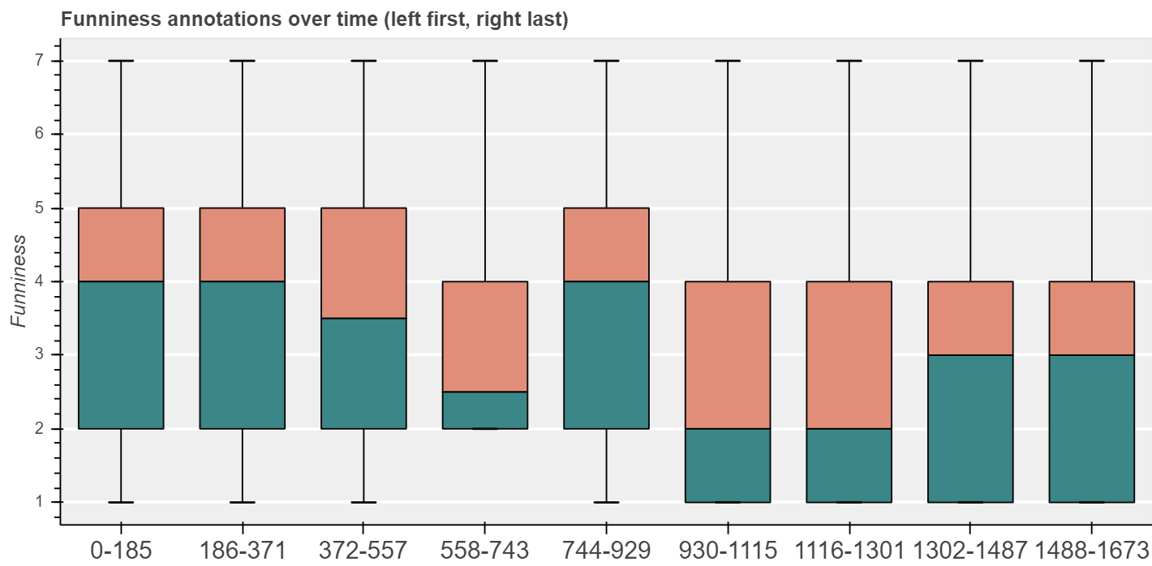
\includegraphics[width=1.0\textwidth]{graphics/average_funniness_over_time}
	\caption{Box plots of the average funniness over time}
	\label{fig:boxplottime}
\end{figure}

A word count analysis showed that there are significant difference in the frequency of certain words. These words seem to contain certain connections to a cartoon theme. For example one of the most frequent words for funniness class 7 is "Thag" which is a common name for cartoons set in the stone age. A similar phenomena could also be observed for word phrases. For example the phrase "thousand more year" is also primarily associated with cartoons set in the stone age. A model could learn this preferences and use it to predict the funniness of a cartoon. For detailed plots please refer to figure [\ref{fig:wordocc1}], [\ref{fig:wordocc2}], [\ref{fig:phraseocc1}] and [\ref{fig:phraseocc2}].

\begin{figure}
\centering

\begin{subfigure}[b]{0.45\textwidth}
\centering
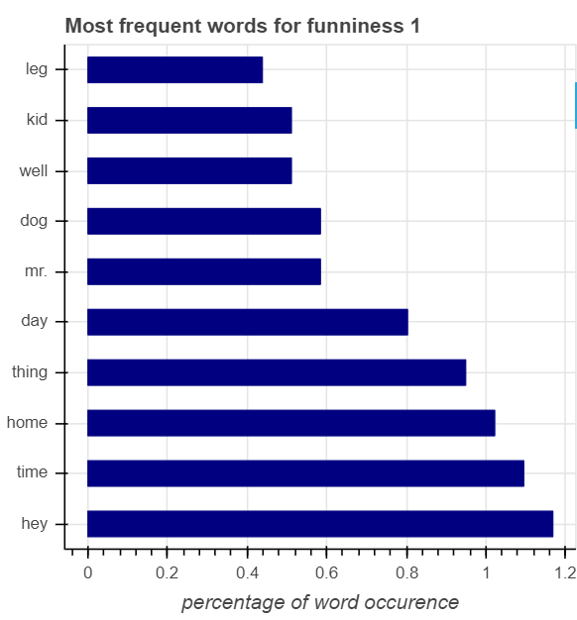
\includegraphics[width=1.0\textwidth]{graphics/word_occurence/funniness_1}
\end{subfigure}\quad
\begin{subfigure}[b]{0.45\textwidth}
\centering
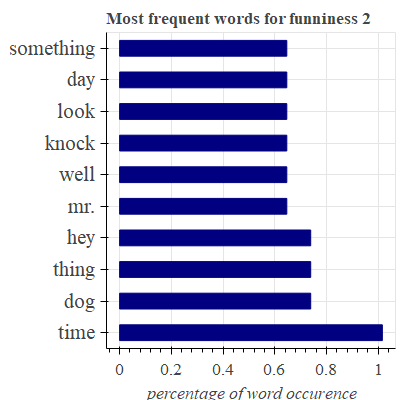
\includegraphics[width=1.0\textwidth]{graphics/word_occurence/funniness_2}
\end{subfigure}

\begin{subfigure}[b]{0.45\textwidth}
\centering
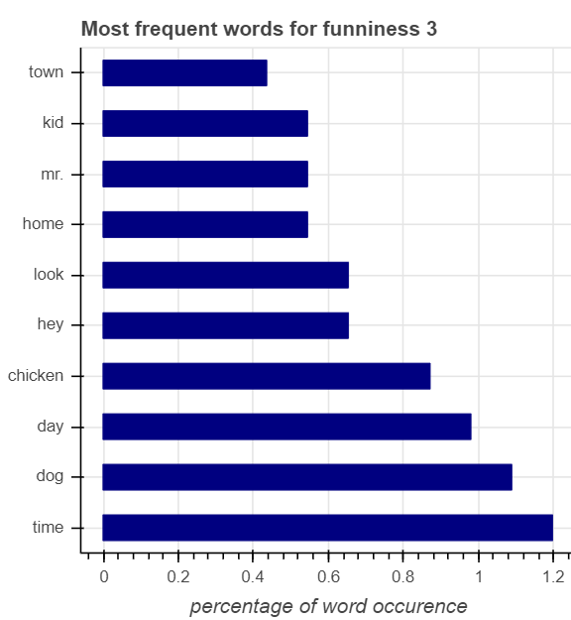
\includegraphics[width=1.0\textwidth]{graphics/word_occurence/funniness_3}
\end{subfigure}\quad
\begin{subfigure}[b]{0.45\textwidth}
\centering
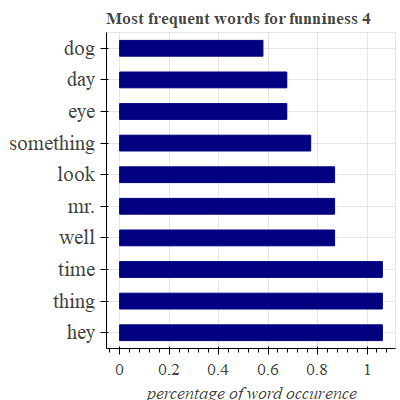
\includegraphics[width=1.0\textwidth]{graphics/word_occurence/funniness_4}
\end{subfigure}


\caption{Most frequent nouns per class 1, 2, 3 and 4.}
\label{fig:wordocc1}

\end{figure}

\begin{figure}
\centering

\begin{subfigure}[b]{0.45\textwidth}
\centering
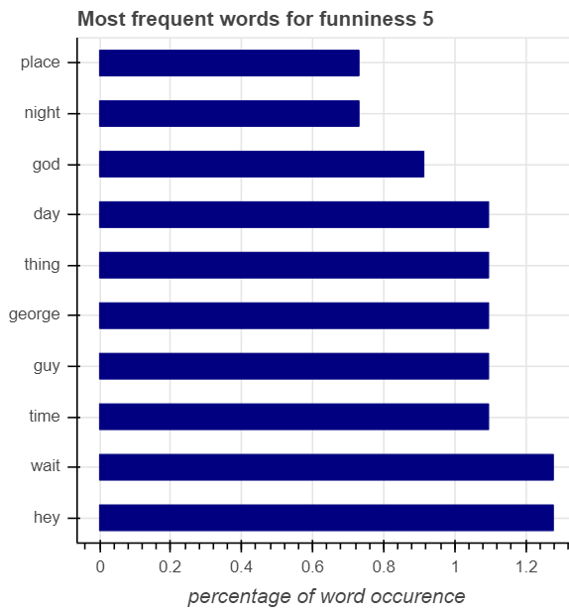
\includegraphics[width=1.0\textwidth]{graphics/word_occurence/funniness_5}
\end{subfigure}\quad
\begin{subfigure}[b]{0.45\textwidth}
\centering
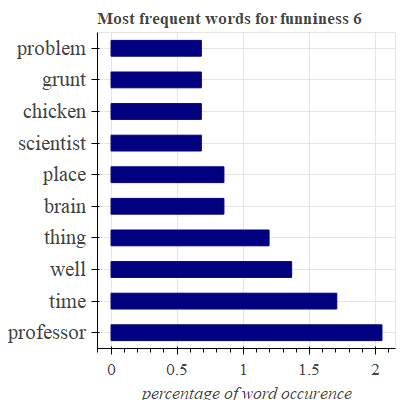
\includegraphics[width=1.0\textwidth]{graphics/word_occurence/funniness_6}
\end{subfigure}


\begin{subfigure}[b]{0.45\textwidth}
\centering
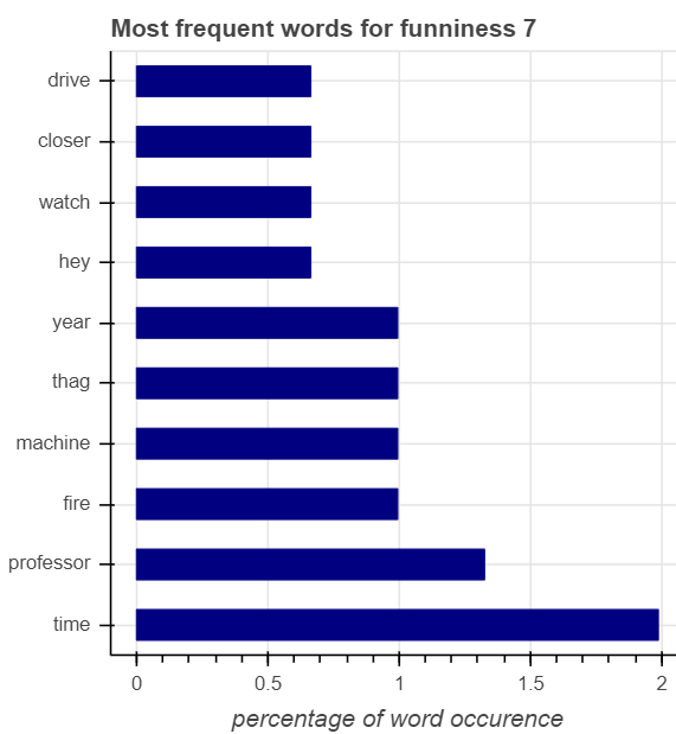
\includegraphics[width=1.0\textwidth]{graphics/word_occurence/funniness_7}
\end{subfigure}

\caption{Most frequent nouns per class 5, 6 and 7.}
\label{fig:wordocc2}

\end{figure}

\begin{figure}
\centering

\begin{subfigure}[b]{0.45\textwidth}
\centering
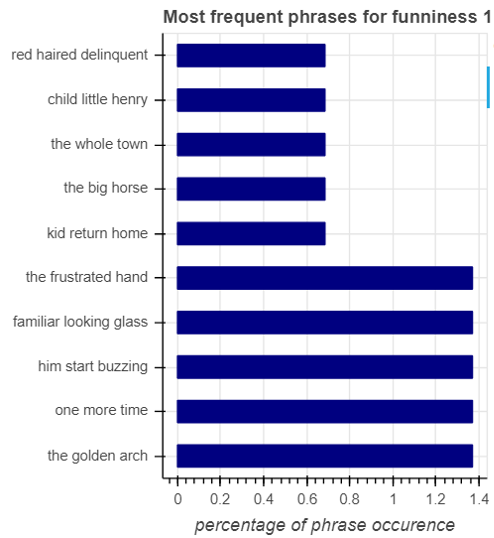
\includegraphics[width=1.0\textwidth]{graphics/phrases/funniness_1}
\end{subfigure}\quad
\begin{subfigure}[b]{0.45\textwidth}
\centering
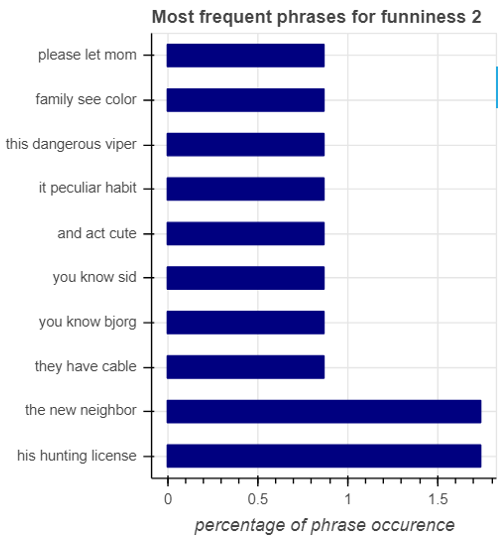
\includegraphics[width=1.0\textwidth]{graphics/phrases/funniness_2}
\end{subfigure}

\begin{subfigure}[b]{0.45\textwidth}
\centering
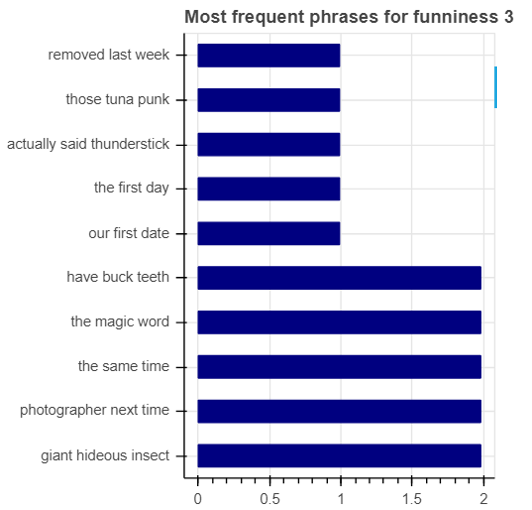
\includegraphics[width=1.0\textwidth]{graphics/phrases/funniness_3}
\end{subfigure}\quad
\begin{subfigure}[b]{0.45\textwidth}
\centering
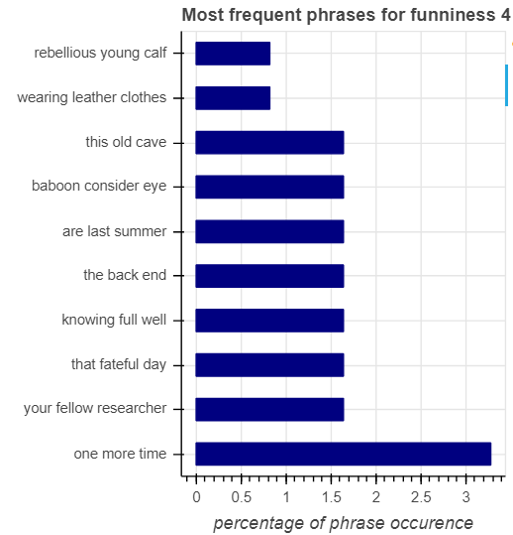
\includegraphics[width=1.0\textwidth]{graphics/phrases/funniness_4}
\end{subfigure}


\caption{Most frequent phrases per class 1, 2, 3 and 4.}
\label{fig:phraseocc1}

\end{figure}

\begin{figure}
\centering

\begin{subfigure}[b]{0.45\textwidth}
\centering
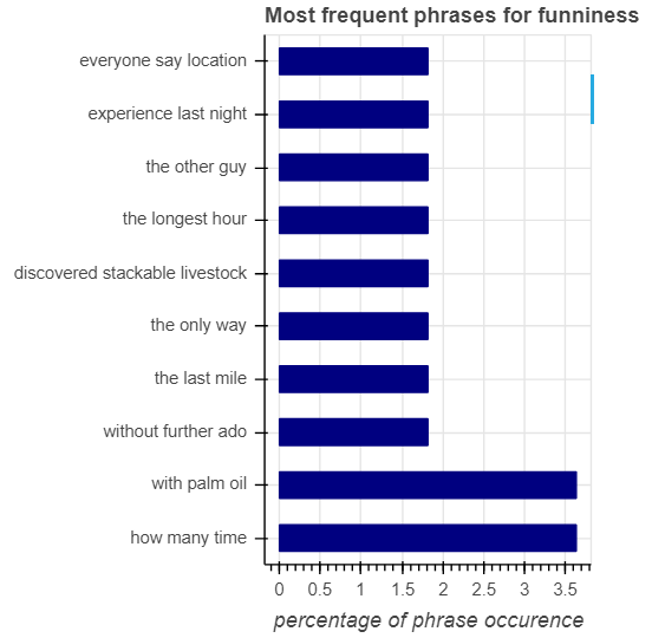
\includegraphics[width=1.0\textwidth]{graphics/phrases/funniness_5}
\end{subfigure}\quad
\begin{subfigure}[b]{0.45\textwidth}
\centering
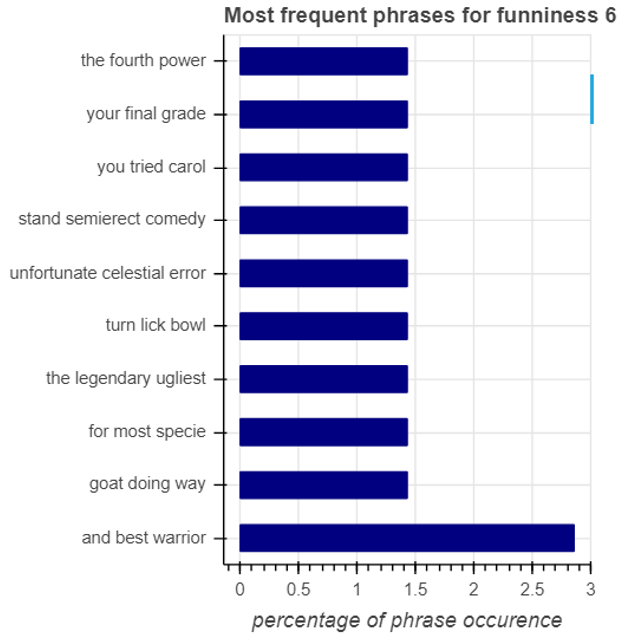
\includegraphics[width=1.0\textwidth]{graphics/phrases/funniness_6}
\end{subfigure}


\begin{subfigure}[b]{0.45\textwidth}
\centering
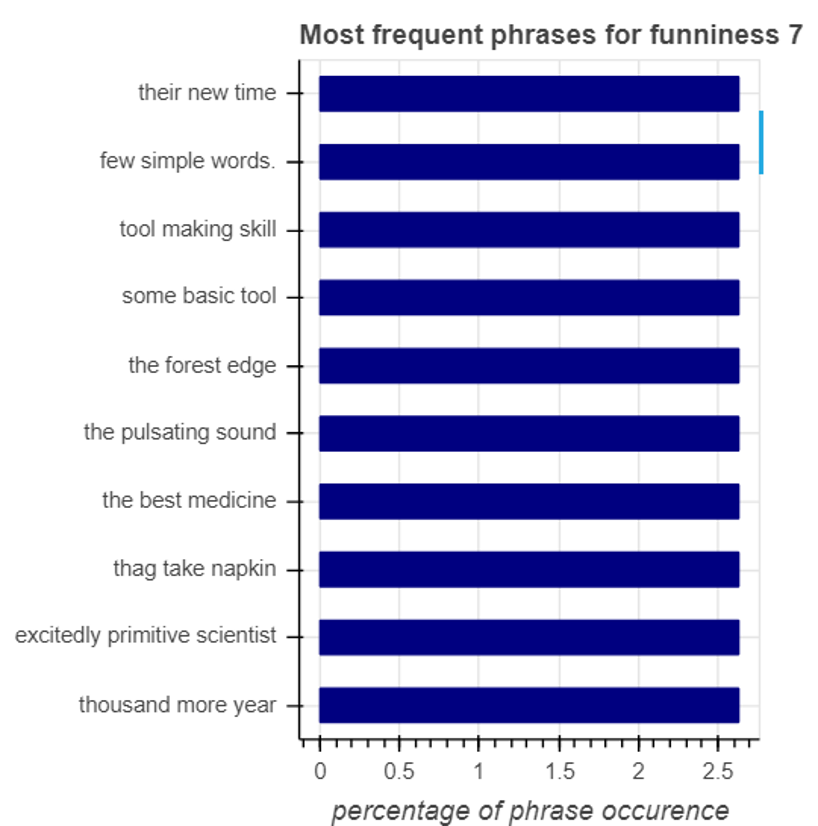
\includegraphics[width=1.0\textwidth]{graphics/phrases/funniness_7}
\end{subfigure}

\caption{Most frequent phrases per class 5, 6 and 7.}
\label{fig:phraseocc2}

\end{figure}


\section{Architectures}
Several architectures have been implemented and are evaluated in the following sections.


\subsection{Baseline}

Four baseline strategies have been selected: 

\begin{itemize}

\item Most Frequent Baseline: Picks the most frequent label in the dataset.
\item Average Baseline: Returns the average funniness of the dataset. For the accuracy metric the average is rounded using round to nearest integer.
\item Random Baseline: Returns a random funniness picked uniformly from one to seven.
\item Stratified Baseline: Returns a funniness sampled from the distribution of the
training set.

\end{itemize}

For the mean absolute error metric the average performed best, while for the accuracy
score the most frequent class has the best score.

\subsection{Simple CNN}
The simple CNN architecture overfits very quickly. The accuracy and MAE sores are
very similar to the most frequent baseline, which indicates that the model most likely
learns to return the most frequent class, instead of generalizing the humour.

\subsection{Transfer Learning of Pretrained ResNet18}
Noteworthy about this approach is that also enabling the data augmentation in the
training phase makes this approach better than the baseline. The exact reason is not
obvious, but indicates that the model does not generalize enough for the
training samples which are not augmented.

The data augmented version of this experiment unexpectedly achieved the best results
during testing phase.

\subsection{Transfer Learned Object Detection}

The result of the object detection approach are incomparable to the other results, as it was not implemented far enough to return any labels. Since initial tests for a simplified image classification task, it was not further developed, as the predicted objects for each object were essentially
random.

\subsection{ELMo Pretrained Model}

Based on the pretrained ELMo model this model initially looked the most promising, as it
achieved the highest validation accuracy. Unfortunately this was only due to overfitting,
as during test phase the performance dropped.

One problem of this approach may be, that many insider jokes of Gary Larson's humour are lost.

Most likely a problem of this approach is that many insider jokes are lost, due to the fact
that the pretrained vocabulary of the ELMo model does not contain many of them, so
they can not be used by our model.

\subsection{AutoML Model}
Initially, when testing on the validation set, the TFIDF configuration looked very promising, as it achieved top results with a very simple feature representation. The test set
revealed overfitting. The ELMo feature representation performed worse in both settings.
Since the TFIDF feature representation would not have relied on a pre-trained vocabulary
it would not have suffered by the problem of domain specific words.

For this experiment the library hyperopt-sklearn was used, as it accomplishes state-ofthe-art of AutoML.

\subsection{Two Stage Model}
The Two Stage Models did not achieve significantly improved results, as it was not able
to beat the baseline. The idea of trying to avoid overfitting by splitting the big tasks into
smaller sub networks which only have a binary decision to make did not work as expected.

Combining the visual and textual information also did not work as hoped. The MAE
score is on par with the baseline, while still beating it at the accuracy score - so it is
technically better. The improvement is not strong enough, that to say that it really
understands humour.

One problem identified was the fact, that the images contained much more data and
also much more noise. Do the idea was to use a deep autoencoder, which reduced the
feature size of the images significantly. But against our expectation it did not improve
the results compared to previous attempts.

\subsection{Autoencoder}

The goal of the auto encoder using the deep convolutional architecture is to reduce the dimensionality of the images, while still maintaining the important characteristics of the original cartoons. 

Comparing the reconstructed cartoon with the original cartoon reveals that the autoencoder looses important information which could be crucial for understanding humour. For example the facial expressions are lost, as well as many other high frequency details. For example the native american lying on the floor is not recognizable anymore. 

These details seem to be very important for the funniness classification task and if missing cause the image data to be not more than additional noise, which is probably the reason why the two stage model with autoencoded cartoons performs the worst.

\begin{figure}
	\centering
  	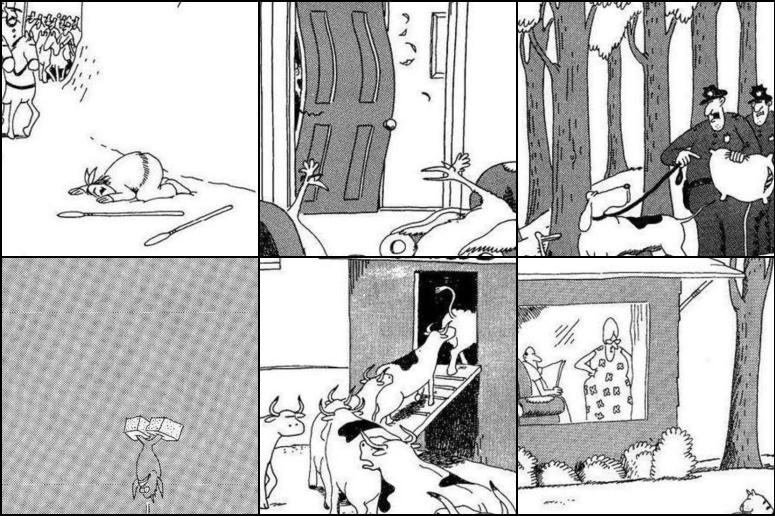
\includegraphics[width=1.0\textwidth]{graphics/autoencoder_original.png}
	\caption{Original Cartoons}
	\label{fig:autoencoderimageoriginal}
\end{figure}

\begin{figure}
	\centering
  	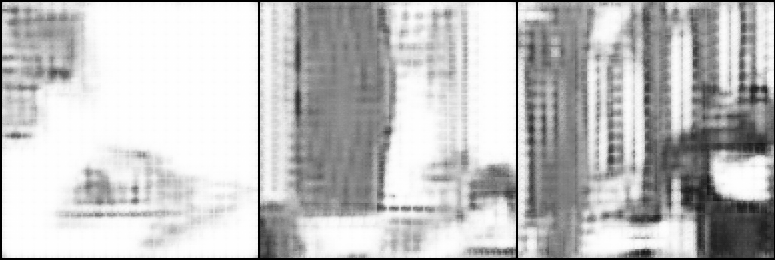
\includegraphics[width=1.0\textwidth]{graphics/autoencoder_final.png}
	\caption{Results after applying encoder and decoder}
	\label{fig:autoencoderresults}
\end{figure}


\section{Detailed Analysis}

Sampling for each class a cartoon and examining the output layer of the trained neural network reveals some insight about the model. In general the results show, that the classifier never assigns high confidence into the predictions. No classification assigns a probability higher than 40\%.

When examining the distribution across the different predictions over the different samples it seems that the general distribution does not change significantly. Some deviations are present, for example when comparing the probabilities for funniness 2.

In general it seems that the model often ignores the input data and instead learns the label distribution. The similarities between the predictions and the histogram of funniness occurrences are very high. Compare figure [\ref{fig:figdistr1}] and figure [\ref{fig:figdistr2}] with figure [\ref{fig:labeldistr}].



\begin{figure}
\centering

\begin{subfigure}[b]{0.45\textwidth}
\centering
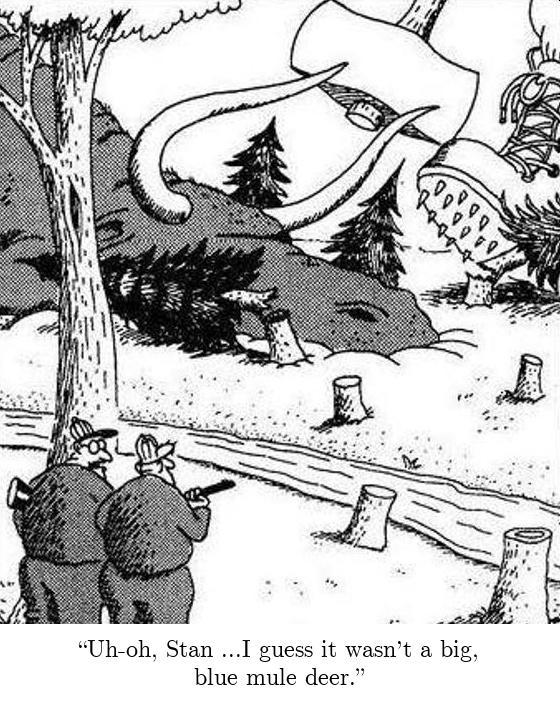
\includegraphics[width=0.9\textwidth,height=0.3\textheight,keepaspectratio]{graphics/detail/Test_for_Image_1_cartoon} \\
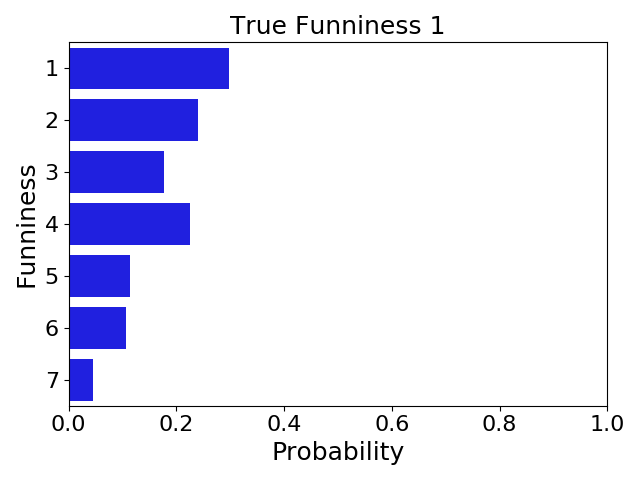
\includegraphics[width=1.0\textwidth]{graphics/detail/Test_for_Image_1}
\end{subfigure}\quad
\begin{subfigure}[b]{0.45\textwidth}
\centering
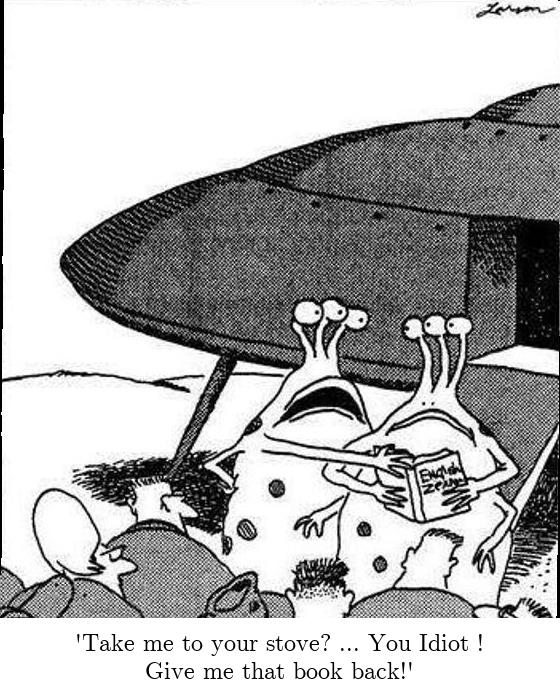
\includegraphics[width=0.9\textwidth,height=0.3\textheight,keepaspectratio]{graphics/detail/Test_for_Image_2_cartoon} \\
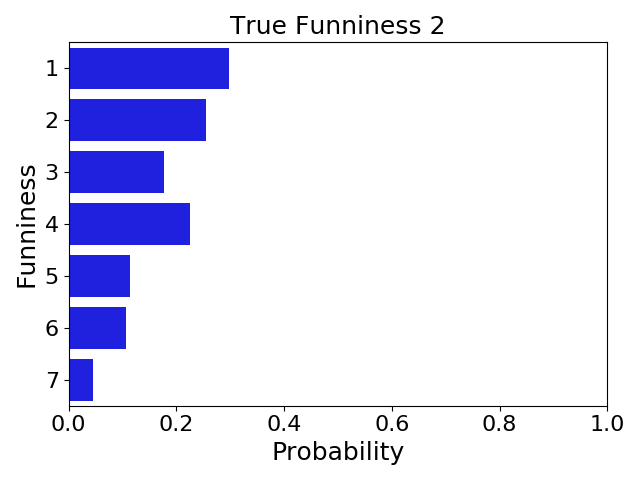
\includegraphics[width=1.0\textwidth]{graphics/detail/Test_for_Image_2}
\end{subfigure}

\begin{subfigure}[b]{0.45\textwidth}
\centering
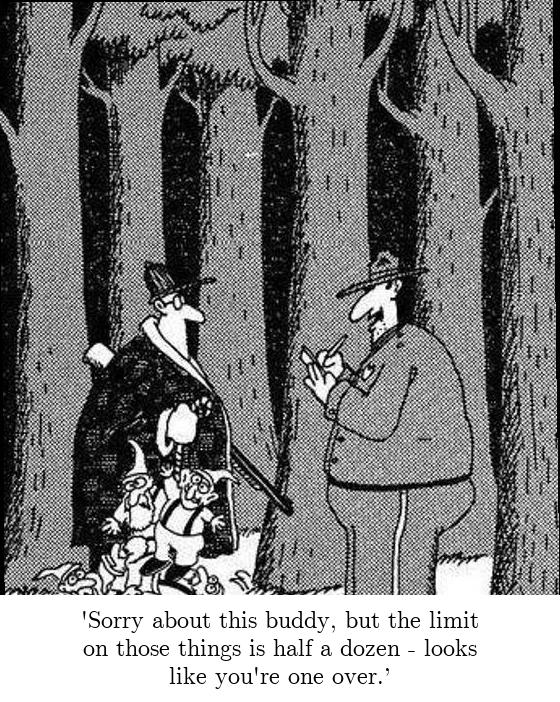
\includegraphics[width=0.9\textwidth,height=0.3\textheight,keepaspectratio]{graphics/detail/Test_for_Image_3_cartoon} \\
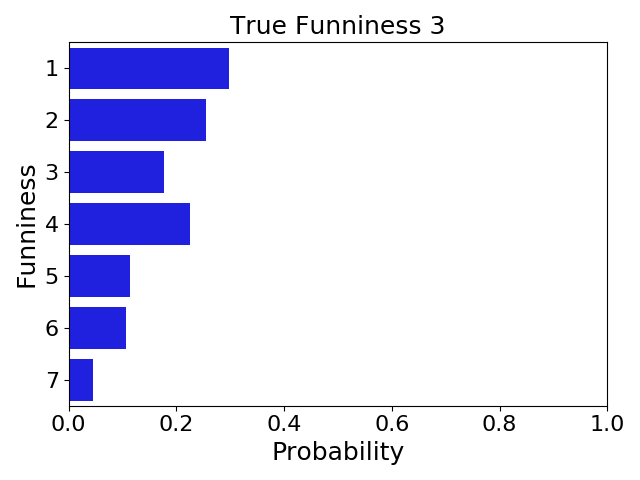
\includegraphics[width=1.0\textwidth]{graphics/detail/Test_for_Image_3}
\end{subfigure}\quad
\begin{subfigure}[b]{0.45\textwidth}
\centering
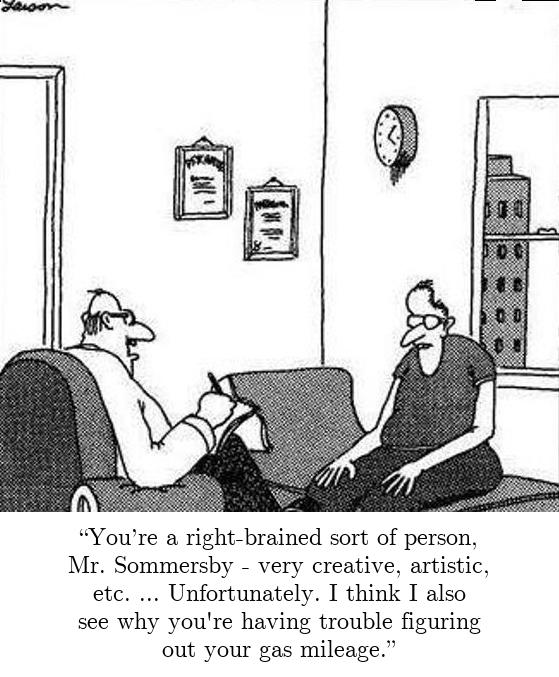
\includegraphics[width=0.9\textwidth,height=0.3\textheight,keepaspectratio]{graphics/detail/Test_for_Image_4_cartoon} \\
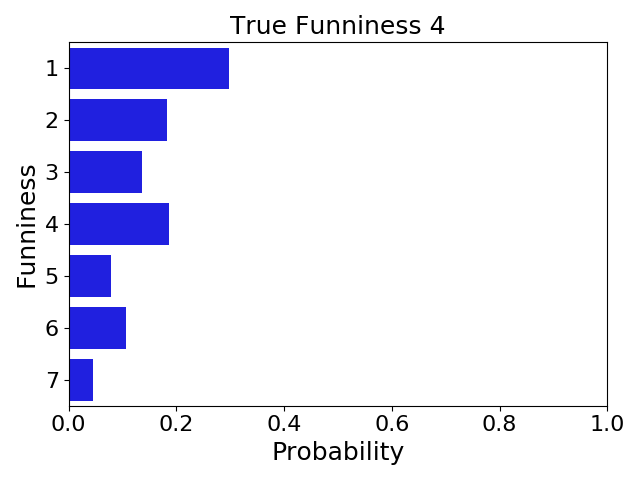
\includegraphics[width=1.0\textwidth]{graphics/detail/Test_for_Image_4}
\end{subfigure}

\caption{For the classes 1, 2, 3 and 4: The bar plots represent the probability the classifier assigned each category for the cartoon above.}

\label{fig:figdistr1}

\end{figure}


\begin{figure}
\centering

\begin{subfigure}[b]{0.45\textwidth}
\centering
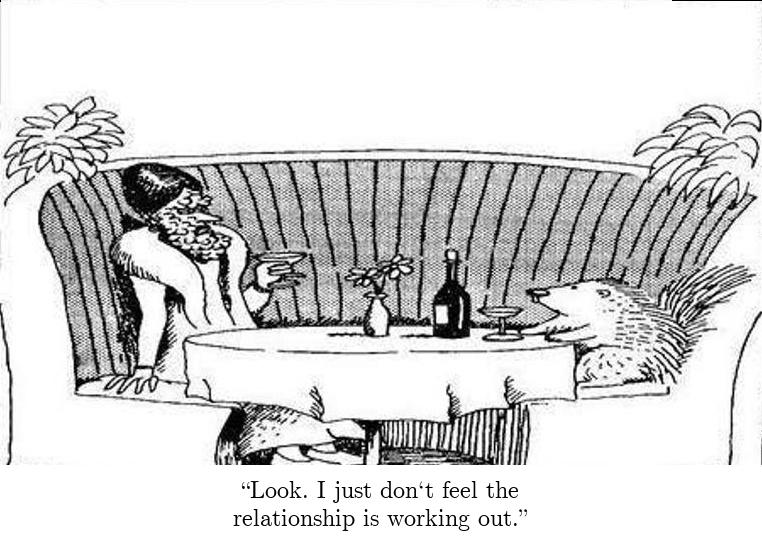
\includegraphics[width=0.9\textwidth,height=0.3\textheight,keepaspectratio]{graphics/detail/Test_for_Image_5_cartoon} \\
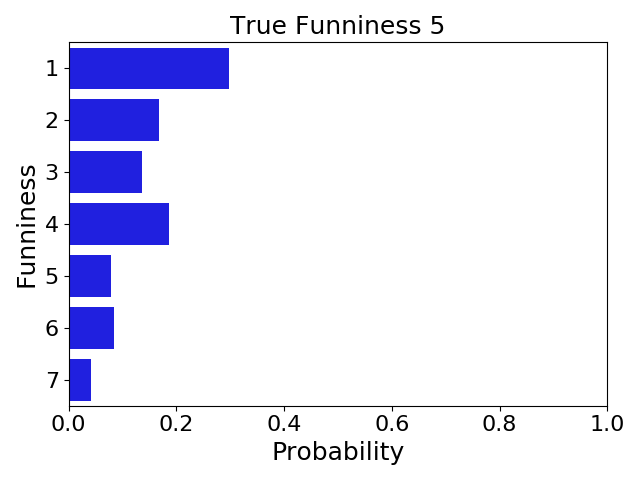
\includegraphics[width=1.0\textwidth]{graphics/detail/Test_for_Image_5}
\end{subfigure}\quad
\begin{subfigure}[b]{0.45\textwidth}
\centering
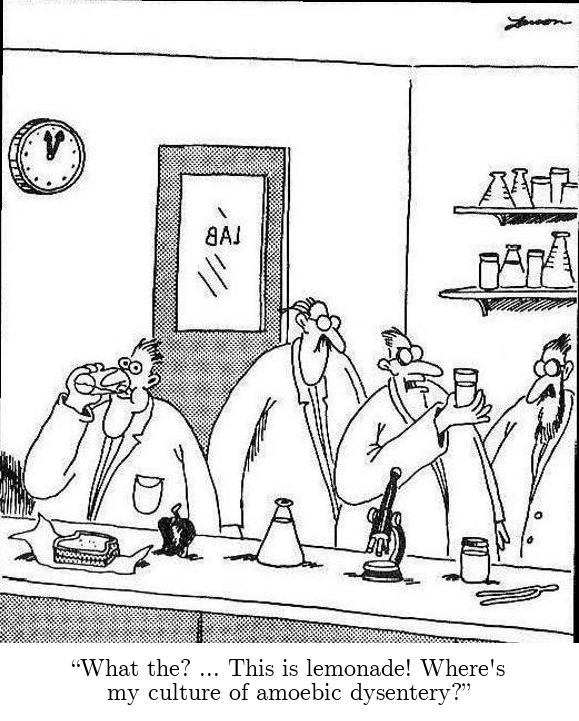
\includegraphics[width=0.9\textwidth,height=0.3\textheight,keepaspectratio]{graphics/detail/Test_for_Image_6_cartoon} \\
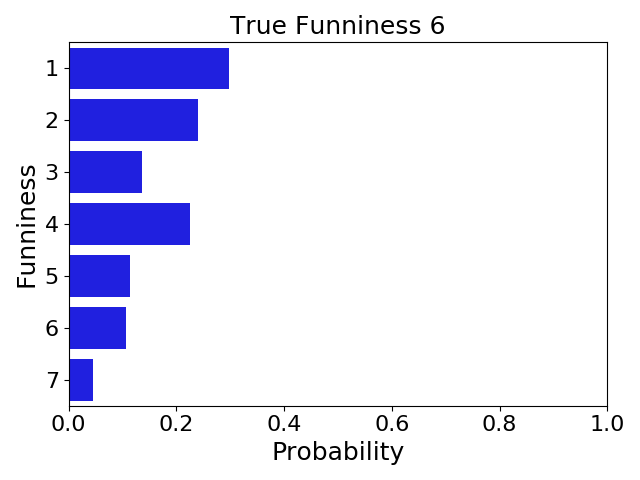
\includegraphics[width=1.0\textwidth]{graphics/detail/Test_for_Image_6}
\end{subfigure}

\begin{subfigure}[b]{0.45\textwidth}
\centering
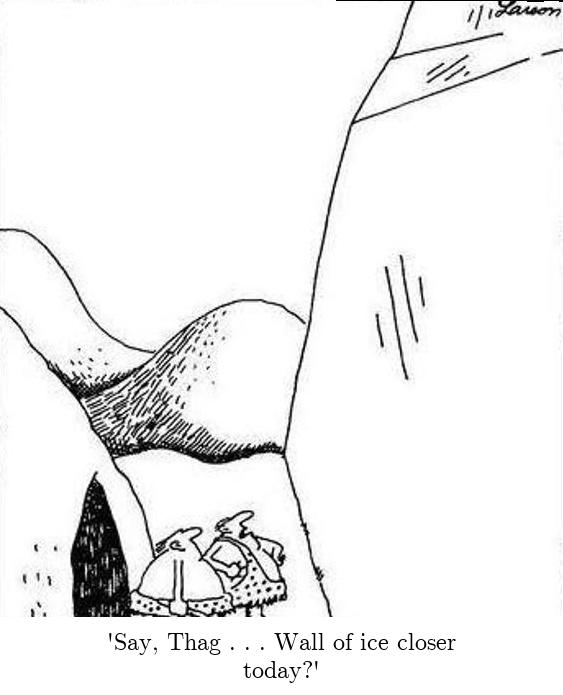
\includegraphics[width=0.9\textwidth,height=0.3\textheight,keepaspectratio]{graphics/detail/Test_for_Image_7_cartoon} \\
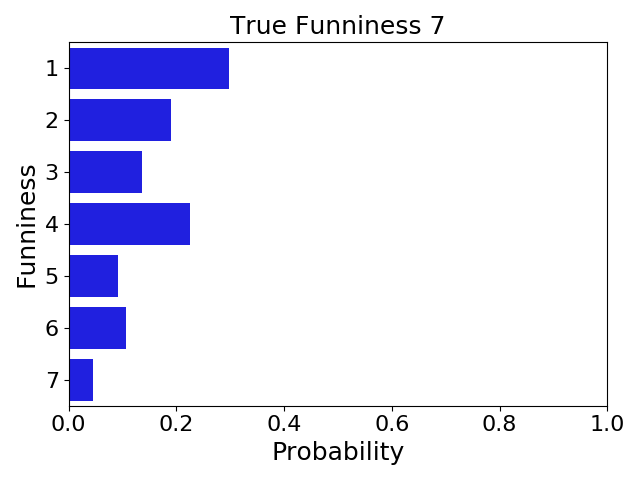
\includegraphics[width=1.0\textwidth]{graphics/detail/Test_for_Image_7}
\end{subfigure}\quad
\caption{Continued for the classes 5, 6 and 7.}
\label{fig:figdistr2}

\end{figure}

\begin{figure}
	\centering
  	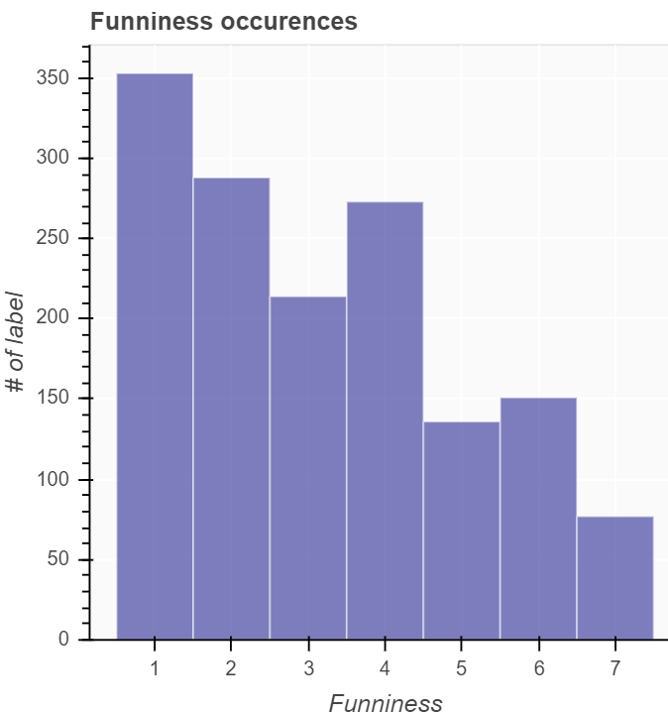
\includegraphics[width=0.75\textwidth]{graphics/label_distribution.png}
	\caption{The label distribution of the training set}
	\label{fig:labeldistr}
\end{figure}


\subsubsection{Confusion Matrix}
\begin{figure}
	\centering
  	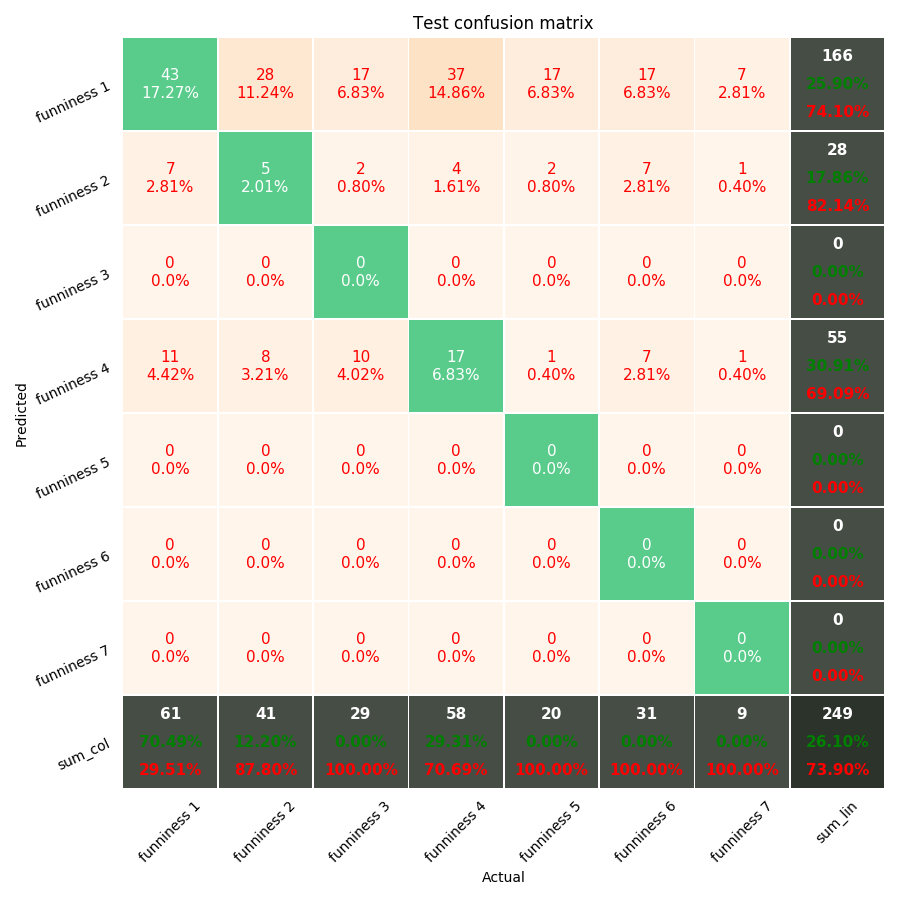
\includegraphics[width=1.0\textwidth]{graphics/transfer_confusion_test.png}
	\caption{Confusion Matrix of the transfer learning CNN (with data augmentation) on the test split}
	\label{fig:confusionmatrixtransferlearningtest}
\end{figure}

\begin{figure}
	\centering
  	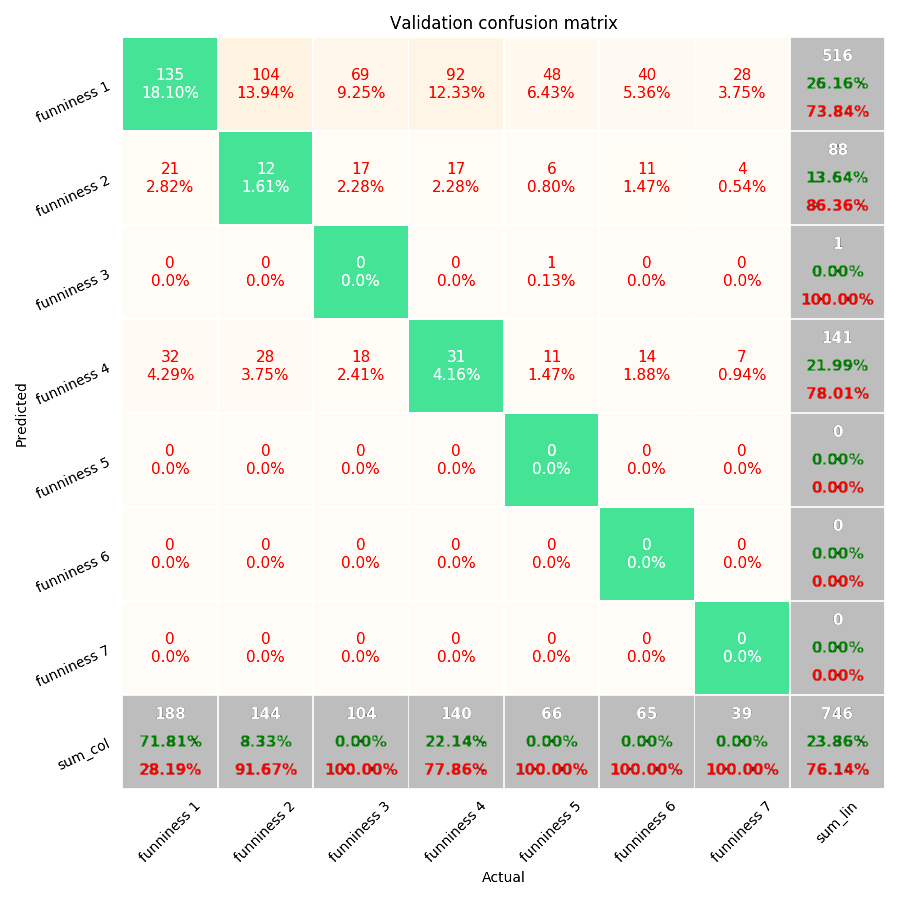
\includegraphics[width=1.0\textwidth]{graphics/transfer_confusion_val.png}
	\caption{Confusion Matrix of the transfer learning CNN (with data augmentation) on the validation split}
	\label{fig:confusionmatrixtransferlearningval}
\end{figure}

One can clearly see that for both the validation and test split the model learned to approximate the label distribution, instead of learning to generalize the underlying structure. The three most frequent funniness classes (1, 4 and 2) are the only ones the model predicts and are therefore by chance correct. Other classes are not predicted at all by the classifier. This motivated the design of the two stage model where the first stage trained a neural network for each class. The task for this neural is to determine whether the given sample belongs to the funniness class it belongs to or not. The second stage uses these results and outputs a final prediction.

When comparing the MAE of the Two stage model (figure [\ref{twostagemae}]) an interesting phenomena can be observed: Even though the performance is very similar to the average baseline, the actual MAEs per class are different.

\begin{figure}
\centering
\begin{tabular}{|l|l|l|l|l|l|l|l|} 
\hline
\textbf{Funniness} 	& \textbf{1}	& \textbf{2}	& \textbf{3}	& \textbf{4}	& \textbf{5}	& \textbf{6}	& \textbf{7}  \\ 
\hline
Two Stage Model     & 2.42			&  1.57			& 0.97			& 0.8			& 1.53			& 2.28			& 3.64   \\
Baseline Average    & 2.21			& 1.21			& 0.21			& 0.79			& 1.79			& 2.79			& 3.79 \\	
\hline
\end{tabular}
\caption{MAE per class}
\label{twostagemae}
\end{figure}

\section{Additional Experiments}
Honourable mention of experiments performed but did not make the cut for an analysis, in no particular order:

\begin{itemize}
\item \textbf{LSTM / GRU}: Overfitting was a big problem early on
\item \textbf{Wasserstein Loss instead of Cross Entropy Loss}: Idea was to penalize near misses less compared to big misses, similar to the regression L1 loss.
\item \textbf{Applying a discrete cosine transformation (DCT)}: Since convolutions are not well suited for line drawings the idea was to apply a DCT beforehand. 
\item \textbf{Advanced Two Stage Model}: Add different binary classifiers in the first stage.
\item \textbf{Loss Weighting of Two Stage Model}: Try different penalties for different kind of errors in the first stage. For example add more penalty for true positives compared to false negatives.
\item \textbf{Preprocessing of cartoons}: Apply different filters on cartoons. For example: Canny edge detection.
\item \textbf{Word vector combinations}: Many different word vector combinations of TFIDF, SpaCy and ELMo. 
\end{itemize}

\section{Results}

The following sections show the achieved performance for each experiment of the validation
and test phase. Additionally the training runtime is also listed.


\subsection{Validation Results}

For a detailed table of validation performance of selected models, please refer to figure [\ref{fig:valperformance}]. The ELMo based model achieved on this subset the highest accuracy, while the Two Stage Model achieved the best Mean Absolute Error. Both models only use the text data and discard the visual information entirely.

\begin{figure}
\begin{tabular}{|l|l|l|l|l|}
\hline
\textbf{Experiment}                                                                       & \textbf{\begin{tabular}[c]{@{}l@{}}Validation\\   MAE\end{tabular}} & \textbf{\begin{tabular}[c]{@{}l@{}}Validation\\   Accuracy\end{tabular}} & \textbf{Text} & \textbf{Visual} \\ \hline
Baseline Most Frequent                                                                    & 2.14                                                                & 25.20\%                                                                  &               &                 \\
Baseline Average                                                                          & 1.53                                                                & 13.94\%                                                                  &               &                 \\
Baseline Random                                                                           & 2.33                                                                & 13.81\%                                                                  &               &                 \\
Baseline Stratified                                                                       & 2.03                                                                & 16.62\%                                                                  &               &                 \\
Simple CNN                                                                                & 2.14                                                                & 25.20\%                                                                  &               & \cmark               \\
Transfer Learning CNN                                                                      & 1.88                                                                & 25.53\%                                                                  &               & \cmark               \\
\begin{tabular}[c]{@{}l@{}}Transfer Learning CNN (with\\   data augmentation)\end{tabular} & 1.96                                                                & 23.86\%                                                                  &               & \cmark               \\
ELMo                                                                                      & 1.81                                                                & \textbf{26.81\%}                                                                  & \cmark             &                 \\
AutoML Model with ELMo Vectors                                                            & 2                                                                   & 25.87\%                                                                  & \cmark             &                 \\
\begin{tabular}[c]{@{}l@{}}AutoML Model with TFIDF\\   Vectors\end{tabular}               & 2.05                                                                & 26.76\%                                                                  & \cmark             &                 \\
Two Stage Model                                                                           & \textbf{1.52}                                                                & 18.10\%                                                                  & \cmark             & \\
Two Stage Model with Cartoons                                                             & 1.55                                                                & 15.68\%                                                                  & \cmark             & \cmark               \\
\begin{tabular}[c]{@{}l@{}}Two Stage Model with\\   Autoencoded Cartoons\end{tabular}     & 1.62                                                                & 15.82\%                                                                  & \cmark             & \cmark               \\ \hline
\end{tabular}
\caption{Model performances on the validation set.}
\label{fig:valperformance}
\end{figure}

\subsection{Test Results}

The results at figure [\ref{fig:testperformance}] show the performance of the models for the test set. Compared to the validation set the best performing models change: The model which maximizes the accuracy measure is now using the visual data, namely the transfer learning CNN on the data augmented test set. Also the two stage model with cartoon data seems to generalize slightly better.

\begin{figure}
\begin{tabular}{|l|l|l|l|l|}
\hline
\textbf{Experiment}                                                                       & \textbf{Test MAE} & \textbf{Test Accuracy} & \textbf{Text} & \textbf{Visual} \\ \hline
Baseline Most Frequent                                                                    & 2.26              & 24.50\%                &               &                 \\
Baseline Average                                                                          & \textbf{1.57}              & 11.65\%                &               &                 \\
Baseline Random                                                                           & 2.17              & 13.65\%                &               &                 \\
Baseline Stratified                                                                       & 2.22              & 14.46\%                &               &                 \\
Simple CNN                                                                                & 2.26              & 24.50\%                &               & \cmark               \\
Transfer Learning CNN                                                                      & 1.96              & 24.90\%                &               & \cmark               \\
\begin{tabular}[c]{@{}l@{}}Transfer Learning CNN (with\\   data augmentation)\end{tabular} & 2.01              & \textbf{26.10\%}                &               & \cmark               \\
ELMo                                                                                      & 1.84              & 25.70\%                & \cmark             &                 \\
AutoML Model with ELMo Vectors                                                            & 2.12              & 24.50\%                & \cmark             &                 \\
\begin{tabular}[c]{@{}l@{}}AutoML Model with TFIDF\\   Vectors\end{tabular}               & 2.23              & 24.90\%                & \cmark             &                 \\
Two Stage Model                                                                           & 1.6               & 18.80\%                & \cmark             &                 \\
Two Stage Model with Cartoons                                                             & \textbf{1.57}              & 16.06\%                & \cmark             & \cmark               \\
\begin{tabular}[c]{@{}l@{}}Two Stage Model with\\   Autoencoded Cartoons\end{tabular}     & 1.58              & 14.46\%                &\cmark             & \cmark              \\
\hline
\end{tabular}
\caption{Model performances on the test set.}
\label{fig:testperformance}
\end{figure}

\subsection{Training Duration}

Figure [\ref{trainingruntime}] shows the training durations of each experiment. A general trend, is that the text based models (ELMo, Two Stage Model) train significantly faster than the visual based models (Simple CNN, Transfer Learning CNN, Two Stage Model with Cartoons). This can be explained by the size of the input vector for the neural network. The data for the text representation is denser for the text representation compared to the representation of images.

\begin{figure}
\centering
\begin{tabular}{|l|l|} 
\hline
\textbf{Experiment}                                    & \textbf{Train Duration}  \\ 
\hline
Baseline Most Frequent                        & \textless{}1s   \\
Baseline Average                              & \textless{}1s   \\
Baseline Random                               & \textless{}1s   \\
Baseline Stratified                           & \textless{}1s   \\
Simple CNN                                    & 7m 50s          \\
Tranfer Learning CNN                          & 15m 45s         \\
Tranfer Learning CNN (with data augmentation) & 9m 52s          \\
ELMo                                          & 4m 39s          \\
AutoML Model with ELMo Vectors                & 29m 7s          \\
AutoML Model with TFIDF Vectors               & 24m 20s         \\
Two Stage Model                               & 8m 42s          \\
Two Stage Model with Cartoons                 & 39m 42s         \\
Autoencoder                                   & 32m 34s         \\
Two Stage Model with Autoencoded Cartoons     & 15m 23s         \\
\hline
\end{tabular}
\caption{Training runtime of each experiment}
\label{trainingruntime}
\end{figure}

\section{Evaluation Conclusion}

In general the conclusion is that no model really learns to generalize the humour of
Gary Larson. There is no significant improvement compared to the baselines available.
Further research into this direction could reveal significant insights into the human humour, as current methods are not capable to achieve significant results.

Potential causes can not be attributed to exactly one issue. One reason is certainly, that the problem space is not sufficiently described by the data set. As most deep learning data sets are many order of magnitudes larger, while the task at hand is arguably easier (For example.: CIFAR 10 data set) than humour classification. Current techniques of transfer learning are not sufficient to solve this issue. Most certainly once more sophisticated transfer learning techniques have been established, solving this problem could be more feasible. 

One could also argue that the problem itself is flawed. Letting a human rate a
cartoon is very subjective and likely depends on many factors. For example: Current mood, whether the person has already seen the cartoon, time of day and also the exact reason for doing the rating. It could be that these factors outweigh the true humour, which makes it impossible to reproduce the original ratings. To answer these questions an additional experiment could be performed. After some time after the initial ratings have been done, the same person rates them again. If and how the results are reproducible could then be evaluated by comparing the results of the new rating versus the old ratings. If the results are much different, this would mean that the problem itself is flawed.

%\chapter{Introduction}
%\todo{Enter your text here.}

%\chapter{Additional Chapter}
%\todo{Enter your text here.}

\backmatter

% Use an optional list of figures.
% \listoffigures % Starred version, i.e., \listoffigures*, removes the toc entry.

% Use an optional list of tables.
% \cleardoublepage % Start list of tables on the next empty right hand page.
% \listoftables % Starred version, i.e., \listoftables*, removes the toc entry.

% Use an optional list of alogrithms.
% \listofalgorithms
% \addcontentsline{toc}{chapter}{List of Algorithms}

% Add an index.
% \printindex

% Add a glossary.
% \printglossaries

% Add a bibliography.
\bibliographystyle{abbrv}
\bibliography{citations.bib}

\end{document}